% Panel (b) of the hearing figure, split from fig-hearing.tex so the paper can present it as a
% subfigure (the (a)/(b) labels now come from LaTeX subcaptions, not baked into the image).
\documentclass[tikz,border=3pt]{standalone}
\usepackage{pgfplots}\pgfplotsset{compat=1.18}
\usepackage{times}
\begin{document}
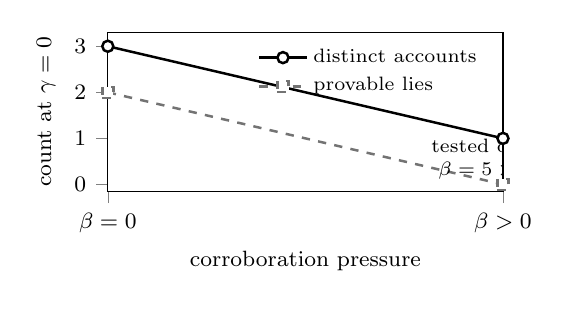
\begin{tikzpicture}
\begin{axis}[font=\footnotesize, width=6.6cm, height=3.6cm,
  xmin=0, xmax=1, xtick={0,1},
  xticklabels={$\beta=0$,$\beta>0$}, xlabel={corroboration pressure},
  tick align=outside, tick pos=left,
  every axis plot/.append style={line width=0.9pt},
  ymin=-0.15, ymax=3.3, ytick={0,1,2,3}, ylabel={count at $\gamma=0$},
  legend style={font=\scriptsize, at={(0.97,0.97)}, anchor=north east, draw=none, fill=none},
  legend cell align=left]
\addplot[black, mark=*, mark options={fill=white}] coordinates {(0,3) (1,1)};
\addlegendentry{distinct accounts}
\addplot[black!55, dashed, mark=square*, mark options={fill=white}] coordinates {(0,2) (1,0)};
\addlegendentry{provable lies}
\node[font=\scriptsize, align=center, anchor=center] at (axis cs:1,0.55)
  {tested down to\\$\beta=5\times10^{-4}$};
\end{axis}
\end{tikzpicture}
\end{document}
